% !TEX root = ../proj_report_outline.tex

\chapter{Three-way Tensors}\label{C:tens}

In order to represent functions of two arguments with neural networks, three-way tensors are 
unavoidable. They have been used, directly or indirectly in a number of highly
successful architectures, often without regard for the underlying structure and interpretation of the
operation. In this chapter we discuss the vector-tensor-vector bilinear product seen in 
eq.~\eqref{eq:grbm} and used implicitly throughout successful multiplicative architectures.

This product admits a surprising
number of interpretations including theorem~\ref{thm:xor} -- that it allows us to operate on a
pair-wise exclusive-or of features. This is a powerful result which shows that admitting tensors
into neural networks can solve the exclusive-or problem without any hidden units. Further, we
demonstrate the expressive power of the tensor by showing that a polynomially sized two layer
network with a
single tensor product is capable of expressing a class of functions which standard two layer networks
can not approximate accurately without exponential size.

The downside of these tensors is the storage requirements. We discuss a well-known method for
expressing the tensor as a product of much smaller matrices and
finally conduct experiments to show that
learning the coefficients of a decomposed tensor can be done in situ with gradient descent.

\section{Definitions}
Formally, we refer to a multi-dimensional array which requires \(n\) indices to address a single
(scalar) element as a \(n\)-way tensor, \(n\) is often referred to as the number of dimensions or modes
of the tensor. A matrix is then a two-way tensor and a vector
a one-way tensor although we will use their usual names for clarity. Notationally, we follow
\autocite{Kolda2009} deviating only where it would become unwieldy.
We denote tensors with three or more dimensions with single calligraphic boldface letters such
as \(\tensor{W}\). Matrices and vectors will be denoted with upper and lower case boldface letters
while scalars will be standard lower case letters. We will often need to address particular
substructures of tensors. This is analogous to pulling out individual rows or columns of a matrix.
To perform this we fix some of the indices to specific values and allow the remaining indices to vary
across their range. We denote by \(\midbullet\) the indices allowed to vary, the rest will be provided
with a specific value. For example, \(\mat{A}_{i \midbullet}\) would denote the \(i\)-th row of the
matrix \(\mat{A}\).
For three-way tensors we refer to the vector elements produced by fixing two indices as 
\emph{threads}. It is also possible to form matrices by fixing only one index -- we refer to these
as \emph{slices}. Table~\ref{tab:notation} in the appendix provides examples.


When dealing with tensor-tensor products, it is important to be precise as there are often
a number of possible permutations of indices that would lead to a valid operation. The downside of
this is that it leads to unwieldy notation. Fortunately, we are only concerned with a few of
special cases. In particular, we need to multiply a three-tensor by a vector and a matrix by a
vector. Matrix-vector multiplication consists of taking the dot product of the vector with
each row of the matrix. For example, with a matrix \(\mat{A} \in \mathbb{R}^{m \times n}\) and a
vector \(\vec{x} \in \mathbb{R}^n\), if \(\vec{y} = \mat{A}\vec{x}\) (with \(\vec{y}\) necessarily
in \(\mathbb{R}^m\)), then
\begin{equation}\label{eq:matmul}
	y_i = \sum_j^n A_{ij} x_j
		= \langle \vec{A}_{i \midbullet}, \vec{x}\rangle
\end{equation} where \(\langle \cdot, \cdot \rangle\) denotes the inner (dot) product. This can be viewed
as taking all of the vectors formed by fixing the first index of \(\mat{A}\) and allowing the second
to vary and computing their inner product with \(\vec{x}\). To perform the same operation using the
columns of \(\mat{A}\) we need to fix the second index, which can be done by exchanging the
order: \(\tran{\vec{x}}\mat{A}\). This kind of operation is sometimes referred to as a
\emph{contractive} product, especially in the physical sciences \autocite{Orus2014}. This name
arises because we form the output by joining a shared dimension (by element-wise multiplication) and
contracting it with a sum.

We can generalise the operation to tensors: choose an index over which to perform the product,
collect every thread formed by fixing all but that one index and take their inner product with the
given vector. If the tensor has \(n\) dimensions, the result will have \(n-1\). A three tensor is in
this way reduced to a matrix. Kolda and Bader introduce the operator
 \(\;\cdot \bar{\times}_i \cdot\;\)
for this, where \(i\) represents the index to vary \autocite{Kolda2009}. For the bilinear forms
we are concerned with, this leads to the following notation:
\begin{align}
	\vec{z} &= \tensor{W} \;\bar{\times}_1\; \vec{x}\; \bar{\times}_2\; \vec{y},
	\implies z_j = \sum_i \sum_k W_{ijk}x_iy_k.
	\label{eq:bilinearkolda}
\end{align}
When \(\tensor{W}\) is a three-way tensor, we prefer a more compact notation
\begin{equation}\label{eq:bilintensor}
	\vec{z} = \tran{\vec{x}}\tensor{W}\vec{y}.
\end{equation} This loses none of the precision of the more verbose notation provided we make clear
that we intend \(\vec{x}\) to operate along the first dimension of the tensor and \(\vec{y}\) the
third. With either notation, for a tensor 
\(\tensor{W} \in \mathbb{R}^{n_1 \times n_2 \times n_3}\), we must have 
\(\vec{x}\in \mathbb{R}^{n_1}\), \(\vec{y} \in \mathbb{R}^{n_3}\) and the result 
\(\vec{z}\in\mathbb{R}^{n_2}\).

\begin{figure}
	\centering
	\begin{subfigure}[t]{0.31\textwidth}
	\centering
	\begin{tikzpicture}
		\draw (0,0) node {} -- (-1,0);
	\end{tikzpicture}
	\caption{Vector \(\vec{a}\in\mathbb{R}^{n_1}\)}\label{fig:tnd:vec}
	\end{subfigure} \hfill
	\begin{subfigure}[t]{0.31\textwidth}
	\centering
	\begin{tikzpicture}
		\draw (1,0) -- (0,0) node {} -- (-1,0);
	\end{tikzpicture}
	\caption{Matrix \(\mat{B}\in\mathbb{R}^{n_1 \times n_2}\)}\label{fig:tnd:mat}
	\end{subfigure}\hfill
	\begin{subfigure}[t]{0.31\textwidth}
	\centering
	\begin{tikzpicture}
		\draw (0,0) node {}
			\foreach \x in {0,90,180}
			{
				(\x:1) -- (0,0)
			};
	\end{tikzpicture}
	\caption{Three-way tensor\\ 
		\(\tensor{C}\in\mathbb{R}^{n_1\times n_2\times n_3}\)}\label{fig:tnd:3ten}
	\end{subfigure}
	\caption{Example tensor network diagrams.}
	\label{fig:tnegs}
\end{figure}

An intuitive way to illustrate these ideas is using Tensor Network Diagrams
\autocite{Cichocki2016, Orus2014}. In these diagrams, each object is represented
as a circle, with each free `arm' representing an index used to address elements.
A scalar has no free arms, a vector one, a matrix two and so on.
Figure~\ref{fig:tnegs} provides examples for these simple objects. 
These diagrams represent a contractive product by joining the
respective arms. As an example, a matrix-vector product \(\vec{y} = \mat{Ax}\)
has such a contraction by eq.~\eqref{eq:matmul}, shown in
figure~\ref{fig:tnmatvec} -- it is clear that there is only a single free arm, so the
result is a vector as it should be. Figure~\ref{fig:tnprods} shows some examples
of these kinds of products.

\begin{figure}
	\centering
	\begin{subfigure}[t]{0.45\textwidth}
		\centering
		\begin{tikzpicture}
			\draw
				(1,0) node (A){} -- (0,0) node(y) {} 
				-- (-1,0);
			\node[below=1em of A, fill=none, draw=none, anchor=mid] {\(\mat{A}\)};
			\node[below=1em of y, fill=none, draw=none, anchor=mid] {\(\vec{y}\)};
		\end{tikzpicture}
		\caption{Matrix-vector product \(\mat{A}\vec{y}\), one free arm indicates
		 the result is a vector.}
		 \label{fig:tnmatvec}
	\end{subfigure} \hfill
	\begin{subfigure}[t]{0.45\textwidth}
		\centering
		\begin{tikzpicture}
			\draw
				(-1,0) node(x){} -- 
				(0,0) node(A) {} --
				(1,0) node(y){};
			\node[below=1em of x, fill=none, draw=none, anchor=mid] {\(\tran{\vec{x}}\)};
			\node[below=1em of A, fill=none, draw=none, anchor=mid] {\(\mat{A}\)};
			\node[below=1em of y, fill=none, draw=none, anchor=mid] {\(\vec{y}\)};
		\end{tikzpicture}
		\caption{Vector-matrix-vector bilinear form \(\tran{\vec{x}}\mat{A}
				 \vec{y}\). No free arms so the result is a scalar.}
	\end{subfigure}\\
	\begin{subfigure}[t]{0.45\textwidth}
		\centering
		\begin{tikzpicture}
			\draw (0,0) node(W) {}
				(180:1) -- node[above, fill=none, draw=none]{\(n_1\)} (0,0)
				(0:1) node(y){} -- node[above, fill=none, draw=none]{\(n_3\)} (0,0)
				(90:1) -- node[above right=1em, fill=none, draw=none]{\(n_2\)} (0,0);
			\node[below=1em of W, fill=none, draw=none, anchor=mid] {\(\tensor{W}\)};
			\node[below=1em of y, fill=none, draw=none, anchor=mid] {\(\vec{y}\)};
		\end{tikzpicture}
		\caption{Tensor-vector product producing a matrix.}
	\end{subfigure} \hfill
	\begin{subfigure}[t]{0.45\textwidth}
		\centering
		\begin{tikzpicture}
			\draw (0,0) node(W) {}
				(180:1) node(x){} -- node[above, fill=none, draw=none]{\(n_1\)} (0,0)
				(0:1) node(y){} --node[above, fill=none, draw=none]{\(n_3\)}  (0,0)
				(90:1) -- node[above right=1em, fill=none, draw=none]{\(n_2\)} (0,0);
			\node[below=1em of x, fill=none, draw=none, anchor=mid] {\(\tran{\vec{x}}\)};
			\node[below=1em of W, fill=none, draw=none, anchor=mid] {\(\tensor{W}\)};
			\node[below=1em of y, fill=none, draw=none, anchor=mid] {\(\vec{y}\)};
		\end{tikzpicture}
		\caption{Vector-tensor-vector product produces a vector.}
		\label{fig:vanillabilintnd}
	\end{subfigure}
	\caption{Various products expressed as Tensor Network Diagrams.}
	\label{fig:tnprods}
\end{figure}

\section{Interpreting Bilinear Products}\label{sec:tensorinterps}
There are several ways to describe the operation performed by the bilinear products we are
concerned which correspond to different interpretations of the results. The following
interpretations provide insight both into what is actually being calculated and how the product might
be applicable in a neural network setting. In all of the below we use the previous definitions of
\(\vec{x}, \vec{y}, \vec{z}\) and \(\tensor{W}\).

\subsection{Stacked bilinear forms}
If we consider the expression for a single element of \(\vec{z}\) in eq.~\ref{eq:bilinearkolda}, 
we can re-write this in terms of the slices of \(\tensor{W}\) as
\(\label{eq:singlezslice}
	z_j = \tran{\vec{x}}\tensor{W}_{\cdot j \cdot}\vec{y}.
\) This reveals the motivation behind the notation in eq.~\eqref{eq:bilintensor}
and shows each element of \(\vec{z}\) is linear  in \(\vec{x}\) or \(\vec{y}\) if
the other is held constant.

This provides an interpretation
in terms of similarities. If we consider the standard dot product of two vectors 
\(\vec{a}\) and
\(\vec{b}\) of size \(m\): 
\begin{equation}
\langle\vec{a}, \vec{b}\rangle = 
\vec{a}^\mathsf{T}\vec{b}
= \sum_{i=1}^ma_ib_i
 = {\cos\theta}{\cdot||\vec{a}||_2\cdot||\vec{b}||_2} 
\end{equation} where
\(\theta\) is the angle in the angle between the vectors. If the dot product
is positive the two vectors are pointing in a similar direction and if it is negative they
are in opposing directions. If it is exactly zero, they must be orthogonal. The dot product
therefore provides us with a measure of the similarity between two vectors.
Indeed if we normalise the vectors by dividing each component by their \(l_2\) norm we
recover exactly the widely used cosine similarity, common in information retrieval 
\autocite{Singhal2001, Tan2006}.

We can generalise this idea by inserting a matrix of (potentially learned)
weights \(\mat{U}\) which enables us
to define general scalar bilinear forms
\begin{equation}
	\langle\vec{a}, \mat{U}\vec{b}\rangle = \langle\vec{a}^\mathsf{T}\mat{U}, \vec{b}\rangle
	= \vec{a}^\mathsf{T}\mat{U}\vec{b}.
\end{equation} In a bilinear tensor product, each component of the result has this form.
As a matrix-vector multiplication consists of
taking the dot product of the vector with each row or column of the matrix
we can also
interpret a matrix-vector multiplication as computing the similarity of the vector with each
row or column of the matrix. 

We can think of the rows of the matrix \(\mat{U}\) 
as containing patterns to look for in the \(\vec{b}\) vector and the columns to
contain patterns to look for in the \(\vec{a}\) vector. If we consider the vectors 
\(\vec{a}\) and \(\vec{b}\) to come from different feature spaces, the matrix \(\mat{U}\)
provides a conversion between them allowing us to directly compare the two. We can therefore
interpret each coordinate of the result of the bilinear tensor product as being an
independent similarity measure based on different interpretations of the underlying
feature spaces. In this sense, where a matrix multiplication looks for patterns in a single input
space a bilinear product looks for \emph{joint} patterns in the combined input spaces of
\(\vec{x}\) and \(\vec{y}\). This becomes clear if we write out each element of the result
vector
\begin{equation} \label{eq:features}
	\vec{z} = \begin{bmatrix}
		\tran{\vec{x}}\mat{W}_{\midbullet 1 \midbullet}\vec{y} \\
		\tran{\vec{x}}\mat{W}_{\midbullet 2 \midbullet}\vec{y} \\
		\vdots \\
		\tran{\vec{x}}\mat{W}_{\midbullet n_2 \midbullet}\vec{y}
	\end{bmatrix}
	= \begin{bmatrix}
		\langle\vec{x}, \mat{W}_{\midbullet 1 \midbullet} \vec{y}\rangle \\
		\langle\vec{x}, \mat{W}_{\midbullet 2 \midbullet} \vec{y}\rangle \\
		\vdots \\
		\langle\vec{x}, \mat{W}_{\midbullet n_2 \midbullet} \vec{y}\rangle
	\end{bmatrix}
	 = \begin{bmatrix}
	 	\cos \theta_1 \cdot ||\vec{x}||_2 \cdot ||\mat{W}_{\midbullet 1 \midbullet}\vec{y}||_2 \\
	 	\cos \theta_2 \cdot ||\vec{x}||_2 \cdot ||\mat{W}_{\midbullet 2 \midbullet}\vec{y}||_2 \\
		\vdots \\
	 	\cos \theta_{n_2} \cdot ||\vec{x}||_2 \cdot ||\mat{W}_{\midbullet n_2 \midbullet}\vec{y}||_2 \\
	 \end{bmatrix}.
\end{equation}


\subsection{Choosing a matrix}
Following on from the above discussion we claim that for each coordinate of the output we are
computing a \emph{similarity vector} which we compare to the remaining input to generate a
scalar value. If we consider all coordinates at once, we see that this amounts to having
one input choose a matrix of patterns, which we then multiply by the remaining input vector. 
%We have
%refrained from making these points in terms of the specific vectors referenced above to make
%the point that the operation is completely symmetrical. While it aids interpretation to think
%of one vector choosing a matrix for the other vector, we can always achieve the same
%intuition after switching the vectors, give or take some transposes.

This interpretation is clear from the expression of the product in
eq.~\eqref{eq:bilinearkolda}. Simply by inserting parentheses we observe that we are
first generating a matrix dependent on the first input and multiplying
the second input by that matrix.

This intuition of choosing a matrix is suggested in \autocite{Sutskever2013} in the
context of language modelling with RNNs. The suggestion is that allowing the current input
character to choose the hidden-to-hidden weights matrix should allow better use of the context. 
%This intuition (and the proposed factorisation of the tensor) was put to use earlier in
%Conditional Restricted Boltzmann Machines \autocite{Taylor} in a more feed-forward setting.

Although this provides a powerful insight into the bilinear product, it is worth reinforcing that
the product is entirely symmetrical. We can not think purely about it as \(\vec{x}\) choosing a matrix
for \(\vec{y}\) as the converse is equally true.

% MAYBE CUT
\subsection{Tensor as an independent basis}
Extending the above to try and capture the symmetry of the operation, we introduce
the notion that the coefficients of the tensor represent a basis in which to compare the
two inputs, independent of both of them. This idea is explained in
 \autocite{Tenenbaum2000} which considered the problem of data that can be described by two
independent factors.
The tensor then contains a basis which characterises the interaction by which the factors
in the input vectors combine to create an output observation.

To make this concrete
consider the case when both vectors have a single element set to \(1\) and the remainder
\(0\). In this case the first tensor-vector product corresponds to taking a slice of the
tensor, resulting in a matrix. The final matrix-vector product corresponds to picking a
row or column of the matrix. Consequently the whole operation is precisely looking up
a fibre of the tensor. Generalising to vectors of real coefficients, we simply replace the idea of a
\emph{lookup} with that of a \emph{linear combination}. The vectors then represent the coefficients
of weighted sums; first over slices and then over rows or columns. The final product is a
distinct representation of both vectors in terms of the independent basis expressed by the tensor.

\subsection{Operation on the outer product}
The most powerful interpretation arises from the observation that the bilinear product is
a linear operation on pair-wise products of inputs.
This interpretation is essential for understanding the expressive
power of the operation as it gives rise to an obvious exclusive-or behaviour.
A way to approach this interpretation arises from a method of implementing the bilinear 
product in terms of simple matrix operations.

To discuss
this we need to introduce the \emph{matricisation} of a tensor. This
operation is a way of \emph{unfolding} or \emph{flattening} a tensor into a large matrix,
preserving its elements. Specifically we define the mode-\(n\)
matricisation of a tensor as an operation which takes all mode-\(n\) fibres
of the tensor and places them as columns of a matrix. We denote the mode-\(n\)
matricisation of a tensor \(\tensor{W}\) as \(\matr_n(\tensor{W})\). While the operation is
straightforward, describing the exact permutation of the indices is awkward -- 
for the general case see
\autocite{Kolda2009}. 

It is easiest to show with an example. 
Consider the three-way tensor \(\tensor{X} \in \mathbb{R}^{2 \times 3 \times 4}\)
with slices
\begin{align} \label{eq:slicies}
	&\mat{X}_{1 \midbullet \midbullet} = \begin{bmatrix}
		a & d & g & j \\
		b & e & h & k \\
		c & f & i & l \\
	\end{bmatrix},
	&\mat{X}_{2 \midbullet \midbullet} = \begin{bmatrix}
		m & p & s & v \\
		n & q & t & w \\
		o & r & u & x \\
	\end{bmatrix}.
\end{align} To construct \(\matr_2(\tensor{X})\) we fix the first and third indices and place the
resulting threads as columns of a new matrix. Fixing the first index corresponds to choosing one of
these slices while fixing the third amounts to choosing a column of the slice.
The result is:
\begin{equation}\label{eq:matricisedeg}
	\matr_2(\tensor{X}) = \begin{bmatrix}
		a & d & g & j & m & p & s & v \\
		b & e & h & k & n & q & t & w \\
		c & f & i & l & o & r & u & x
	\end{bmatrix}.
\end{equation}

We also require the related \(\vect\) operator from linear algebra.
This flattens a matrix into a vector by stacking its columns. For some matrix \(\mat{A}\) with
\(n\) columns:
\begin{equation}\label{eq:vec}
	\vect(\mat{A}) = \begin{bmatrix}
		{\vec{A}_{\midbullet 1}} \\
		{\vec{A}_{\midbullet 2}} \\
		\vdots \\
		{\vec{A}_{\midbullet n}}
	\end{bmatrix}.%^\mathsf{T}.
\end{equation}

A 
mode-2 matricisation of a
three-way tensor \(\tensor{W} \in \mathbb{R}^{n_1\times n_2\times n_3}\) must have shape
\(n_2 \times n_1n_3\). The following lemma helps us describe the resulting matrix.

\begin{lem}[Matricisation/vectorisation]
The \(j\)-th row of the mode-2 matricisation of the three-way tensor \(\tensor{W}\)
is equivalent to the vectorisation of the transpose of the slice formed by fixing the second index 
at \(j\):
\begin{equation}\label{eq:matlemstatement}
	\matr_2 (\tensor{W})_{j \midbullet} = \vect(\tran{\mat{W}_{\midbullet j \midbullet}}).
\end{equation}
\label{lem:matricise}
\end{lem}
\begin{proof}
By the above definition of the vectorisation operator, each index \((i, k)\) in some matrix
\(\mat{U} \in \mathbb{R}^{n_1\times n_3}\) maps to element \(i + (k-1)n_1\) in
\(\vect(\mat{U})\). By the definition of the mode-2 matricisation we would expect to
find tensor element \(W_{ijk}\) at index \((j, i + (k-1)n_1)\). Hence if we fix \(j\), we have
precisely the vectorisation of the \(j\)-th slice of the tensor.

The indices into \(\matr_2(\tensor{W})\) arise from the following construction.
First fix all indices to 1. Construct a column by sweeping the second index, \(j\),
through its full range. Then increment the first index \(i\) and repeat the procedure, appending
the generated columns to a matrix as we go. Only when \(i\) has covered its full range
increment the final index \(k\) and repeat the procedure. The generated columns should then be
at positions \(i + (k-1)n_1\).
\end{proof}

To understand the lemma it helps to consider an example. Using the \(2 \times 3 \times 4\)
tensor \(\tensor{X}\) defined
in eq.~\eqref{eq:slicies}, fixing the second index to \(2\) gives a \(4 \times 2\) 
transposed slice:
\begin{equation}\label{eq:mode2slice}
	\tran{\mat{X}_{\midbullet 2 \midbullet}} = \begin{bmatrix}
		b & n \\
		e & q \\
		h & t \\
		k & w
	\end{bmatrix}.
\end{equation} Vectorising this matrix takes each column and stacks them, giving
\begin{equation}\label{eq:veceg}
	\vect(\tran{\mat{X}_{\midbullet 2 \midbullet}}) = \begin{bmatrix}
		b &
		e &
		h &
		k &
		n &
		q &
		t &
		w
	\end{bmatrix}^\mathsf{T}
\end{equation} which is precisely row two of eq.~\eqref{eq:matricisedeg}.

These flattenings are important as they allow us to
implement many operations involving tensors in terms of large matrix operations which can be efficiently
parallelised. The next lemma describes how we use a flattened tensor to implement a bilinear product.

\begin{lem}[Matricised product]\label{lem:outerprod}
For a tensor \(\tensor{W}\) and vectors \(\vec{x}\), \(\vec{y}\) as above,
we can describe the product \(\vec{z} = \tran{\vec{x}}\tensor{W}\vec{y}\) in terms of the
mode-2 matricisation of \(\tensor{W}\) as 
follows:
\begin{align}
	\vec{z} = \matr_2(\tensor{W})\mathrm{vec}\left[\vec{y}\tran{\vec{x}}\right]
	\label{eq:bilinearouter}
\end{align}
\end{lem}

\begin{proof}
To
prove this we can compare the expressions for a single element of the result.
An element \(z_j\) from eq.~\eqref{eq:bilinearouter}
is formed as the inner product of the \(j\)-th
row of the flattened tensor and the vectorised outer product of the inputs. By 
lemma~\ref{lem:matricise}:
\begin{equation}
	z_j = 
	\sum_{s=1}^{n_1n_3} \left(\matr(\tensor{W})\right)_{js} \cdot
	\left( \vect\left[\vec{y}\tran{\vec{x}}\right]\right)_s
\end{equation}
We replace the sum over \(s\) with a sum over two
indices, \(i\) and \(k\), and using them to appropriately re-index the flattenings 
as described in lemma~\ref{lem:matricise} we 
derive
\begin{align}
	z_j &= \sum_{i=1}^{n_1}\sum_{k=1}^{n_3} W_{ijk} x_i y_k 
		= \tran{\vec{x}}\mat{W}_{\midbullet j \midbullet}\vec{y}
\end{align}

\end{proof}


Therefore to understand the bilinear product it helps to understand the matrix 
\(\vec{y}\vec{x}^\mathsf{T}\). This matrix takes the following form:
\begin{equation}\label{eq:outer}
	\vec{y}\tran{\vec{x}} = \begin{bmatrix}
		x_1y_1 & \ldots & x_{n_1}y_1 \\
		\vdots & \ddots & \vdots \\
		x_1y_{n_3} & \ldots & x_{n_1}y_{n_3}
	\end{bmatrix}
\end{equation} which contains all possible products of pairs of elements, one from each vector. 
This enables the following result.

\begin{thm} [Bilinear exclusive-or] \label{thm:xor}
Bilinear tensor products operate on the pair-wise exclusive-or of the
signs of the inputs.
\end{thm}
\begin{proof}
Consider the sign of a scalar product
\(c = a\cdot b\). If one of the operands \(a\) or \(b\) is positive and the other negative,
then the sign of \(c\) is negative. If both are positive or both are negative, then the
result is positive. This captures precisely the ``one or the other but not both'' structure
of the exclusive-or operation.

By lemma~\ref{lem:outerprod} a bilinear product can be viewed as a matrix operation on the flattened
outer product of the two inputs. As each element in the outer product is the product of two scalars,
the signs have an exclusive-or structure.
\end{proof}

\begin{cor}[Bilinear conjunctions]\label{cor:and}
If the inputs are binary, bilinear products operate on pair-wise conjunctions of the inputs.
\end{cor}
\begin{proof}
If \(a, b \in \{0, 1\}\), then \(a \cdot b = 1\) if and only if both \(a\) and \(b\) are \(1\). If
either or both are \(0\) then their product must be zero. Following the same structure as the proof
of theorem~\ref{thm:xor}, for binary inputs we must have this conjunctive relationship.
\end{proof}

\subsubsection{Implications of theorem~\ref{thm:xor}:}
\paragraph{Higher level features.}
This indicates that the bilinear tensor products operate implicitly on higher
level features, constructed by combining both inputs. This indicates that it is capable of capturing
complex relationships between both.
\paragraph{XOR.}
The case where both inputs are the same, \(\vec{z} = \tran{\vec{x}}\tensor{W}\vec{x}\),
provides an interesting building block for feed-forward networks. A plain perceptron has been 
long known to be incapable of learning the exclusive-or
mapping \autocite{Minsky1969} -- a neural network to solve the problem requires either a hidden layer
or an additional input feature such as the conjunction of the inputs \autocite{Rumelhart1986}.
By corollary~\ref{cor:and} this quadratic tensor form would capture the
conjunctive feature and be capable of solving the exclusive or problem without hidden
layers or hand-engineered features.
\paragraph{Apparent depth.}
While it has long been known that neural networks with a single hidden layer and
appropriate non-linearity (and therefore two weight matrices)
 are universal function approximators \autocite{Hornik1989}, recent results
have suggested that increased depth allow exponential increases in expressivity for a fixed number
of parameters \autocite{Eldan2016, Telgarsky2016}. We claim that allowing tensor products has the effect
of allowing similar increases without additional hidden layers.
%\end{description}
\paragraph{}
The final claim requires justification.
Eldan and Shamir show that for a
particular class of radial basis-like functions which depend only on the squared norm of the 
input
\footnote{Precisely, functions \(f : \mathbb{R}^n \mapsto \mathbb{R}\) such that
\(f(\vec{x}) = f(\vec{y})\) implies that \(||\vec{x}||^2 = ||\vec{y}||^2\). Eldan and Shamir
deal specifically with cases where the norm is the Euclidean norm (as is the case for the
common squared-exponential kernel). They also
require some additional constraints on the boundedness and support of the function, see
\autocite{Eldan2016} theorem 1, for the precise construction.}
there exist networks with two hidden layers and a number of nodes polynomial in the input dimension
which can perfectly approximate the function. They then show that a shallower network with a single
hidden layer can only perfectly approximate the function with a number of nodes exponential in the
input dimension \autocite{Eldan2016}. This is a very recent result (published in COLT 2016), which
is remarkable as it proves an impossibility: there is a realistic class of functions which it is
impossible to approximate accurately with a two layer network with reasonably bounded size. However,
this restriction can be subverted if we allow tensor semantics in the first layer of the network.

To show this, we first require the following lemma.
\begin{lem}[Squared norm]\label{lem:sqnorm}
	A tensor layer \(\tran{\vec{x}}\tensor{W}\vec{x}\) is capable of exactly computing the squared
	Euclidean norm \(||\vec{x}||^2_2 = \sum_i x_i^2\).
\end{lem}
\begin{proof}
Recalling lemma~\ref{lem:outerprod},
\( \label{eq:outerquad}
	\tran{\vec{x}}\tensor{W}\vec{x} = \matr_2(\tensor{W}) \vect(\vec{x}\tran{\vec{x}}).
\) Note that the diagonal elements of \(\vec{x}\tran{\vec{x}}\) are the components
\(x_i^2\) which we need to sum to compute the squared norm. We simply need to define
\(\matr_2(\tensor{W})\) such that it picks out the correct elements and sums them. If 
\(\vec{x} \in \mathbb{R}^d\) then \(\tensor{W} \in \mathbb{R}^{d \times 1 \times d}\) as we only
require a single output. The matricisation is then a \(1 \times d^2\) row vector and we simply need
to set its elements zero apart from those with indices of the form \(1 + id\) for 
\(i \in \{1, \ldots, d\}\). The matrix product will then simply pick out the elements formerly
on the diagonal and sum them as required.
\end{proof}

\begin{thm}[Exponential expressivity]
There exists a class of functions which can be approximated arbitrarily well by a two layer network
including a single tensor layer with a number of nodes polynomial in the size of the input which
require an exponential number of nodes to be approximated by a standard feed-forward layer.
\end{thm}
\begin{proof}
We make use of Eldan and Shamir's proof \autocite{Eldan2016}. The proof is highly technical so we 
only describe the alterations required to allow a tensor layer.
They construct a three-layer network in the following manner:
for an input \(\vec{x}\), the first two layers learn to approximate the map 
\(\vec{x}\mapsto ||\vec{x}||^2_2 = \sum_i x_i^2\), the final layer learns a univariate function on the
squared norm. Finally, it is show this can be done with layers of polynomial width in the input
dimension.

Using lemma~\ref{lem:sqnorm}, we can compute the squared norm exactly
with a single layer. We can therefore construct a network in
the same fashion as Eldan and Shamir, replacing the first two layers with a single tensor layer. 

This plugs directly into the proof of lemma 10 in \autocite[18--19]{Eldan2016}, simply noting that
we may duplicate the tensor layer a polynomial number of times -- at most we will need the same number of
nodes in the final hidden layer of Eldan and Shamir's three layer network.
\end{proof}

We have shown a single tensor layer can do the work of two feed-forward
layers which provides a strong motivation to explore architectures incorporating these tensor
semantics.


\section{Tensor Decompositions} % should be just CP?
Bilinear products show great promise. Unfortunately
such a tensor is often very large; an \(n \times n \times n\) tensor
would require \(\Theta(n^3)\) space
to store explicitly and a similar number of operations to use to compute a bilinear product. 
This leads to the idea of using a parameterised decomposition -- an ideal solution
would be a method of representing the tensor with some way of specifying the complexity of the
bilinear relationship and hence making explicit the relationship between the number of parameters
required and the expressive power of the model. 

Here we outline and analyse the single most important decomposition. We note that
three-way tensors are something of a special case in which many methods of tensor decomposition
become very closely related. The CP-decomposition discussed here is in many ways the
simplest method yet it retains some very appealing properties. It is also worth observing that
many of the
more complex decompositions were devised to solve the difficulty of finding a CP-decomposition
for a given tensor \autocite{Kolda2009, Hackbusch2009}. This issue does not affect us as we aim
to learn the decomposed tensor in place to model an unknown relation. We are therefore well placed to
prefer the simplicity of the CP. 

The key competition is the Tensor-Train decomposition
\autocite{Osedelets2011}, which has an elegant conceptual interpretation. Unfortunately in the three-way
case it saves relatively little space and proves hard to train compared to the CP. A full discussion
of the differences is deferred to appendix~\ref{A:tt} as the outcome is clear.
We also point the interested reader to Kolda and
Bader's excellent review of the history and applications of a wide range of tensor decompositions
for a full background \autocite{Kolda2009}.

\subsection{CANDECOMP/PARAFAC}
This method of decomposing a tensor dates as far back as 1927 
\autocite{Hitchcock1927, Hitchcock1928} but has been rediscovered repeatedly in a range of
contexts \autocite{Kolda2009}. First referred to as `polyadic
form of a tensor' we refer to it as the CP-decomposition after two prominent publications in
1970 referring to the technique as `canonical decomposition' (CANDECOMP) \autocite{Carroll1970}
 or `parallel factors' (PARAFAC). \autocite{Harshman1970}
 It is a fairly straightforward
extension of a matrix rank decomposition to the more general case, representing a tensor as
a sum of rank one tensors. Some interesting results on the uniqueness of the decompositions can be found
in \autocite{Kolda2009}, but they are not relevant to the discussion here.

\subsubsection{Description}
Given a three-way tensor \(\tensor{X} \in \mathbb{R}^{n_1 \times n_2 \times n_3}\) we wish to 
approximate it as
\begin{equation}\label{eq:cp-statement}
	\tensor{X} \approx \sum_{r=1}^{R} \vec{a}_r \otimes \vec{b}_r \otimes \vec{c}_r
\end{equation}
 where \(R\) is the \emph{rank} of the decomposition and \(\cdot \otimes \cdot\) denotes the tensor
product. This product expands the dimensions; for the first two vectors it is the outer product
\(\vec{a}\tran{\vec{b}}\) which generates a matrix consisting of the product of each pair of
elements in \(\vec{a}\) and \(\vec{b}\). With three such products we proceed analogously, except
now our structure must contain the product of each possible triple of elements. Hence we need
three indices to address each entry, so it is a three-way tensor. Each individual
element has the form
\begin{equation}\label{eq:cp-element}
	X_{ijk} = \sum_{r=1}^R a_{ri}b_{rj}c_{rk}.
\end{equation}

It is convenient to stack these factors into matrices --
we differ slightly from \autocite{Kolda2009} by defining the \textit{factor matrices} of the 
form \(\mat{A} = [\vec{a}_1\;\vec{a}_2\;\cdots\;\vec{a}_R]^{\mathsf{T}} \in 
\mathbb{R}^{R\times n_1}\) (and equivalently for
\(\mat{B}\) and \(\mat{C}\)) such that the  \textit{rows} of the matrix correspond to the
\(R\) vectors. 
We denote a tensor decomposed in this format 
\(\tensor{X} = [\mat{A}, \mat{B}, \mat{C}]_{CP}\).

\subsubsection{Bilinear Product}
We wish to compute a product of the form \(\vec{z} = \tran{\vec{x}}\tensor{W}\vec{y}\)
where \(\tensor{W} = [\mat{A}, \mat{B}, \mat{C}]_{CP}\) is represented as a CP-decomposition.
Conveniently, this can be done with simple matrix products.

\begin{prop} \label{prop:cpbilin}
\begin{align}
	\vec{z} &= \tran{\vec{x}}\tensor{W}\vec{y} 
			= \tran{\mat{B}}(\mat{A}\vec{x} \odot \mat{C}\vec{y})
\end{align}
when \(\tensor{W} = [\mat{A}, \mat{B}, \mat{C}]_{CP}\) and \(\odot\) represents the Hadamard
(element-wise) product.
\end{prop}
\begin{proof}
This follows from straightforward rearranging. Firstly
\begin{align}\label{eq:cpbilin-one}
	z_j &= \sum_{i}^{n_1} \sum_k^{n_3} W_{ijk} x_i y_k 
		= \sum_{i}^{n_1} \sum_k^{n_3} \sum_r^R A_{ri} B_{rj} C_{rk} x_i y_k
		= \sum_r^R B_{rj} \left( \sum_i^{n_1} A_{ri} x_i \cdot \sum_k^{n_3} C_{rk}y_k \right).
\end{align}
We can compute the quantity inside the brackets for all \(r\) at once
by \(\mat{A}\vec{x} \odot \mat{C}\vec{y}\), which results in a length \(R\) vector. 
Equation~\eqref{eq:cpbilin-one} then notes that for each output \(j\) we take the \(j\)-th column
of the \(R \times n_2\) factor matrix \(\mat{B}\) and perform a dot product with our earlier
result. This is naturally expressed by matrix multiplication:
\begin{equation}
	\vec{z} = \mat{B}^\mathsf{T} (\mat{A}\vec{x} \odot \mat{C}\vec{y}).
\end{equation}
\end{proof}

This casts the CP decomposition into a form that looks very similar to some of the
RNNs discussed in chapter~\ref{C:bg}. A key similarity is with the GRU -- the manner in which
the reset gate is applied to the hidden states during the production of the candidate update
\(\vec{z}_t\) could be almost be viewed as a non-linear version of the above.

To express the bilinear product above as a tensor network diagram  we have to insert
an auxiliary \(R\times R\times R\) tensor, denoted \(\tensor{I}_{R}\) which is defined as
\begin{equation}\label{eq:tensoridentity}
	I_{ijk} = \begin{cases}
		1 & \mathrm{if} \; i=j=k, \\
		0 & \mathrm{otherwise}
	\end{cases}
\end{equation} in a manner analogous to the identity matrix. Taking a bilinear product with this
tensor represents element-wise multiplication of the two vectors (see proposition~\ref{prop:identity}
in the appendix). This is
represented diagrammatically with the symbol
\rotatebox[origin=c]{-180}{\(\oslash\)},
shown in 
figure~\ref{fig:cpbilintnd}.

\begin{figure}
	\centering
		\begin{tikzpicture}[scale=0.75]
			\node (0,0) [forbidden sign, 
						 rotate=180, 
						 draw, fill=none, label=above:{\(\tensor{I}\)}] (I) {};
			\draw
				(-2,0) node[label=below:{\(\vec{x}\)}]{}
				 -- (-1,0) node[label=below:{\(\mat{A}\)}]{}
				 -- (I)
				(2,0) node[label=below:{\(\vec{y}\)}]{}
				 -- (1,0) node[label=below:{\(\mat{C}\)}]{}
				 -- (I)
				(I) --
				(0,1) node[label=right:{\(\mat{B}\)}]{}
				 -- (0,2)
			;
		\end{tikzpicture}
	\caption{Bilinear product in the CP-decomposition.}
	\label{fig:cpbilintnd}
\end{figure}

\subsubsection{Discussion}
The CP decomposition does a remarkable job of preserving the expressivity. To illustrate this
consider a special case of the form 
\(
	\tensor{W} = \sum_r^R \vec{a}_r \otimes \vec{e}_r \otimes \vec{c}_r,
\) where \(\vec{e}_i\) are standard basis vectors with all elements zero and
 a one in position \(i\). Consider \(\vec{z} = \tran{\vec{x}}\tensor{W}\vec{y}\). Then
\begin{equation}\label{eq:xorfeatures}
	z_r = \langle \vec{a}_r, \vec{x} \rangle \cdot \langle \vec{c}_r \vec{y}\rangle.
\end{equation} If we apply a sigmoid non-linearity, then \(\sigma(z_r) > 0.5\) implies \(z_r\) is
positive so the dot products must have the same sign. \(\sigma(z_r) < 0.5\) implies \(z_r\) is 
negative. If inserted in a neural network, the CP decomposition has the ability to compute the
exclusive-or of features extracted from the inputs.

Bilinear products with the CP decomposition also retain the ability to express element-wise
multiplication. Recalling the tensor \(\tensor{I} \in \mathbb{R}^{N \times N \times N}\) used
earlier to represent element-wise multiplication,
it is straightforward to model with a CP decomposition:
\(\tensor{I} = [\mat{I}, \mat{I}, \mat{I}]_{CP}\) where \(\mat{I}\) is the 
\(N\times N\) identity matrix. This is can be easily verified as the definition of a bilinear
product with a CP-decomposed tensor includes an element-wise product so it suffices to ensure the
factor matrices do not alter the inputs. The CP-decomposition reduces the required parameters
to \(3N^2\) as opposed to the original \(N^3\). This is a remarkable reduction, considering that
an analogous diagonal \emph{matrix} is the worst case for the corresponding two-way 
decomposition. 

\section{Learning decompositions by gradient descent}
We now present some experimental results 
to verify the expressive power of the decomposed tensor. We justify theoretical
results by showing a tensor layer is capable of solving the exclusive-or problem without hidden units
and then apply it to a real world task to illustrate the benefits of the representation.

\subsection{Gradients}
Before training with gradient descent, we first need to derive the gradients. 
We consider each parameter matrix individually.
As the end goal is the gradient of a vector with respect
to a matrix it should naturally be represented by a three-way tensor of partial derivatives.
Many authors avoid this by
vectorising the matrix \autocite{Magnus2007}, but for the purposes below it is sufficient to note
that the gradients are highly structured, and we can write a simple form for each partial derivative.

Let \(\vec{z}\) be defined as above.
The gradient of \(\vec{z}\) with respect to \(\mat{A}\) has entries of the form:
\begin{align}
	\frac{\partial z_j}{\partial A_{lm}} &= \sum_k^{n_3}B_{lj}C_{lk}x_my_k 
		= B_{lj}x_m \cdot \langle\vec{C}_{l\midbullet}, \vec{y}\rangle.\\
\intertext{The gradients with respect to \(\mat{C}\) are very similar:}
	\frac{\partial z_j}{\partial C_{lm}} &= y_m \cdot \sum_i^{n_1}A_{li}x_i 
		= B_{lj}y_m \cdot \langle\vec{A}_{l\midbullet}, \vec{x}\rangle.\\
\intertext{The gradient of the final parameter matrix \(\mat{B}\) has entries}
	\frac{\partial z_j}{\partial B_{lm}} &= 
		\sum_i^{n_1}\sum_k^{n_3}A_{li}C_{lk}x_iy_k. 
		= \langle\vec{A}_{l\midbullet}, \vec{x}\rangle \cdot 
		\langle\vec{C}_{l\midbullet}, \vec{y}\rangle
		\label{eq:cpbilingrad}
\end{align}
%Curiously, the \(j\) and \(m\) indices do not appear in the right hand side of 
%eq.~\eqref{eq:cpbilingrad}. This appears to suggest that \(\mat{B}\) may learn a significantly
%redundant structure. However, during gradient descent this will be multiplied by the gradient of the
%loss which will be different for each coordinate.

A point to make about these gradients is the prevalence of multiplicative interactions.
This has been noted to occasionally cause problematic dynamics during gradient descent. The
simplest example is to consider
gradient descent on the product of two variables: \(c = ab\). If \(a\) is very small and \(b\) is
very large then the update applied to \(b\) will be very small and the update applied to \(a\) will
be proportionally very large. Sutskever uses this as motivation for using
second-order information during optimisation of RNNs containing similar 
structures \autocite{Sutskever2013}. We prefer to
counsel patience -- after a single step, the gradients will become perfectly aligned to the scale
of the parameters.


\subsection{XOR}
\subsubsection{Goal}
Theoretical results suggest that a single tensor layer should be able to solve the exclusive-or problem.
This is known to be impossible with a single standard
feed-forward layer, so if the tensor layer is successful
in this task it would provide a useful demonstration of the difference in expressive power.

\subsubsection{Experiment Details}
Truth values are represented as binary ones and zeros. 
As there are only four data points, all were evaluated for each parameter update.
All models were trained using standard gradient descent with a learning rate of \(0.5\).

Three models were evaluated: a perceptron (single layer feed-forward network), 
a multi-layer perceptron (MLP) and a single layer tensor. All
models used a sigmoid nonlinearity on the output, the MLP had 4 hidden units also with sigmoids and the 
tensor layer used a rank \(1\) CP decomposition. Models
were trained to minimise the cross-entropy, averaged across the data points with training continuing
for \(1000\) epochs. Although not all MLPs had converged by this time, it was sufficient to see the
difference
between the architectures. To show that the differences are fundamental we repeat the experiments 50
times and observe consistent results.

\subsubsection{Results}
The baseline cross entropy is \(-\log0.5 = 0.6931\), which corresponds to outputting
0.5 for all inputs (or guessing uniformly at random). 
As expected the simple perceptron
converges rapidly to this point. Both the MLP and the tensor are able to solve the task,
although it is interesting to note that the
tensor does so far more rapidly and reliably than the MLP. This is not surprising in light of
corollary~\ref{cor:and} as this is precisely the kind of relationship we would expect the tensor
product to represent naturally.

\begin{figure}
\centering
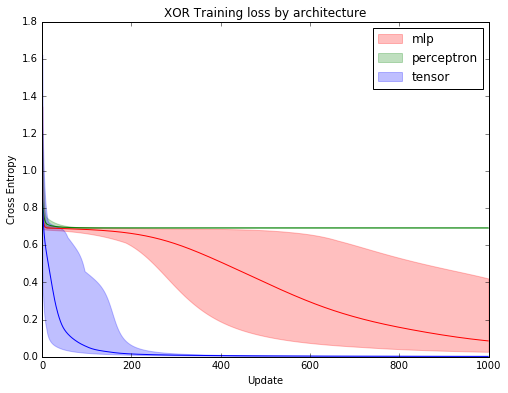
\includegraphics[width=0.45\textwidth]{tensors/xor}
 \caption[XOR results]{Exclusive-or results. Bold line is the mean of 50 runs, shading indicates the
minimum and maximum across all runs.}
\end{figure}

\subsection{Separating Style and Content}
\subsubsection{Goal}
In this section we apply the tensor decompositions to a less trivial task. In particular, we
address the \textit{extrapolation} problem presented by Tenenbaum and 
Freeman \autocite{Tenenbaum2000}. The focus in this task in on data that is naturally presented as a
function of two factors, termed \emph{style} and \emph{content}. Tennenbaum and Freeman
propose the use of bilinear models for such data to naturally capture 
interactions in the joint space of the two
factors. Our aim for reproducing a similar experiment is to verify that we
can learn in place tensor decomposition that represents an unknown, complex relationship.

\subsubsection{Problem Formulation}
Let \(\vec{y}_{sc}\) be an observation vector with style \(s\) and content \(c\). It is modelled
in bilinear form:
\begin{equation}
	\vec{y}_{sc} = \tran{\vec{a}_s}\tensor{W}\vec{b}_c
\end{equation} where \(\vec{a}_s\) and \(\vec{b}_c\) are style and content parameter vectors
respectively and \(\tensor{W}\) represents a set of basis functions independent of the parameters.
A number of tasks involving learning such a model were proposed, but we focus on extrapolation:
 learning both the parameter vectors and the basis tensor at once in such a way that
the model successfully generalises to style and content pairs not seen during training.

We model the style and content parameter vectors as fixed length, dense vectors with a unique
vector for each style label and each content label. The parameters in these vectors can be
learnt by gradient descent jointly with the tensor \(\tensor{W}\). This is equivalent
to representing each style and content label individually
in a one-of-N encoding (a vector with one value per possible label, all
zero apart from the entry corresponding to the label in question) and multiplying it by
a matrix. We refer to such a matrix as an \emph{embedding matrix} as it embeds a sparse encoding
into a smaller, densely populated space. It is clear that if we
were to attempt to learn the model without these embeddings it would fail completely to
generalise. A bilinear product with two such one-of-\(n\) 
vectors would amount to selecting a single fibre
from the tensor, so the tensor could only ever hope to directly store the training data.
Introducing a decomposition changes this by forcing the elements of the tensor to depend on
one another and incorporating an embedding matrix further forces the tensor to separately model
different modes of interaction.

\subsubsection{Data}
One dataset explored in \autocite{Tenenbaum2000} is typographical -- this provides a natural
source of data defined by two factors: font and character. We refer to the character as the
content and the font as the style. We collected a small dataset of five fonts and their
italic/oblique variants for a total of ten styles. Variation between styles comes from stroke
width, slant and the presence or absence of serifs. From each font the uppercase and lowercase
letters of the English alphabet were extracted, totalling 52 different content labels. Data was
saved as 32 pixel by 32 pixel greyscale images. To represent images as vectors for the purposes
of the above model they are flattened in scanline order: left to right then top to bottom.

\subsubsection{Training Details}
This is a very difficult task as we are expecting the model to produce pictures similar to ones
that have never been seen in training. Further, we are trying to train a model with potentially
thousands of free parameters based only on a few hundred examples. As this suggests, stopping
the model from overfitting was the major challenge. The aim of the experiments was not
necessarily to achieve state-of-the-art performance, but to ensure that using a tensor
decomposition to model non-trivial interactions was a feasible goal.

We use a model with
embeddings of size \(25\) and a rank \(25\) CP-decomposition. This model has 78,350
parameters, while a the explicit \(25 \times 1024 \times 25\) tensor
would have 641,550, an eight fold difference in size. 
We train the model using ADAM \autocite{Kingma2014}, a variant of
stochastic gradient descent which dynamically rescales the step size, to minimise the squared error:
\begin{align}
	E = \sum_{i}^B ||\hat{\vec{y}}_{sc} - \vec{y}_{sc}||_2^2
\end{align} where \(B\) is the number of elements in a batch (we used 26) and
\(\hat{\vec{y}}_{sc} = \vec{a}_s^\mathsf{T}\tensor{W}\vec{b}_c\) is the predicted image. Both
the central tensor and the embedding vectors are updated at every step. A small amount
of \(l_2\) regularisation was found to help prevent overfitting. This involves adding a penalty
term to the loss of the form \(\lambda||\mat{X}||_F^2 = \lambda\sum_i\sum_jX_{ij}^2\) for
each matrix in the model.

\subsubsection{Results}
Figure~\ref{fig:sandc-interp} provides a visual inspection of what the model was able to
learn. Images were generated by finding the style and content labels for a two examples and
linearly interpolating first the content vector and then the style vector, generating an
image with the intermediate vectors at each step. 

The start and end images are not perfect; the model was small and unable to capture the training
data exactly. During experimentation larger models were found to fit the data very well, but 
overfitted rapidly, which is why a smaller model was used for these results.
Intermediate stages of the interpolation indicate that the model has
not simply learned to recall individual pairs of labels. We see that as either the content or
the style shifts from one to another, the elements of the source image which are not shared with
the target fade out and are replaced.

Results on unseen data are shown in figure~\ref{fig:sandc-valid}. These show that the captures
much of the salient information for separating the style and content. In
particular, the general shapes of the letters are roughly appropriate and it has begun to capture
some information about the presence or absence of serifs and general slant.
Figure~\ref{fig:sandc-fail} shows a harder example -- the lowercase `a' has considerable variation
among various fonts and the model is unable to guess what would be appropriate for an unseen
example. 

Overall, these results show the tensor was capable of learning a model for the data.
This suggests that the aim of inserting such tensor products into more complex neural networks
is feasible, reinforcing the promising theoretical results.


\begin{figure}[tp]
	\begin{subfigure}[t]{\textwidth}
	\begin{tabu} to \textwidth {XXXXXXXXXX}
		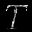
\includegraphics[width=0.09\textwidth]{tensors/sandc/interp/output0} &
		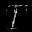
\includegraphics[width=0.09\textwidth]{tensors/sandc/interp/output1} &
		
\includegraphics[width=0.09\textwidth]{tensors/sandc/interp/output2} &
		
\includegraphics[width=0.09\textwidth]{tensors/sandc/interp/output3} &
		
\includegraphics[width=0.09\textwidth]{tensors/sandc/interp/output4} &
		
\includegraphics[width=0.09\textwidth]{tensors/sandc/interp/output5} &
		
\includegraphics[width=0.09\textwidth]{tensors/sandc/interp/output6} &
		
\includegraphics[width=0.09\textwidth]{tensors/sandc/interp/output7} &
		
\includegraphics[width=0.09\textwidth]{tensors/sandc/interp/output8} &
		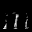
\includegraphics[width=0.09\textwidth]{tensors/sandc/interp/output9} 
	\end{tabu}
	\caption{Linearly interpolating between two content vectors (`T' to `m') with style vector
			 fixed.}
	\end{subfigure}
	\\
	\begin{subfigure}[t]{\textwidth}
	\begin{tabu} to \textwidth {XXXXXXXXXX}
		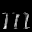
\includegraphics[width=0.09\textwidth]{tensors/sandc/interp/output10} &
		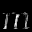
\includegraphics[width=0.09\textwidth]{tensors/sandc/interp/output11} &
		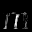
\includegraphics[width=0.09\textwidth]{tensors/sandc/interp/output12} &
		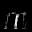
\includegraphics[width=0.09\textwidth]{tensors/sandc/interp/output13} &
		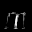
\includegraphics[width=0.09\textwidth]{tensors/sandc/interp/output14} &
		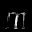
\includegraphics[width=0.09\textwidth]{tensors/sandc/interp/output15} &
		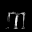
\includegraphics[width=0.09\textwidth]{tensors/sandc/interp/output16} &
		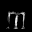
\includegraphics[width=0.09\textwidth]{tensors/sandc/interp/output17} &
		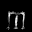
\includegraphics[width=0.09\textwidth]{tensors/sandc/interp/output18} &
		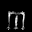
\includegraphics[width=0.09\textwidth]{tensors/sandc/interp/output19}
	\end{tabu}
	\caption{Linearly interpolating between two style vectors with fixed content.}
	\end{subfigure}
	\caption{Learned style and content representations.}
	\label{fig:sandc-interp}
\end{figure}
\begin{figure}[tp]
	\begin{subfigure}[t]{\textwidth}
		\begin{tabu} to \textwidth {XXXXXXXXX}
			
\includegraphics[scale=1]{tensors/sandc/valid/real/Georgia-76} &
			
\includegraphics[scale=1]{tensors/sandc/valid/real/Georgia-77} &
			
\includegraphics[scale=1]{tensors/sandc/valid/real/Georgia-83} &
			
\includegraphics[scale=1]{tensors/sandc/valid/real/VeraMoIt-86} &
			
\includegraphics[scale=1]{tensors/sandc/valid/real/VeraMoIt-100} &
			
\includegraphics[scale=1]{tensors/sandc/valid/real/VeraMoIt-101} &
			
\includegraphics[scale=1]{tensors/sandc/valid/real/VeraMono-66} &
			
\includegraphics[scale=1]{tensors/sandc/valid/real/VeraMono-76} &
			
\includegraphics[scale=1]{tensors/sandc/valid/real/VeraMono-89} 
		\end{tabu}
		\caption{Actual images from the dataset.}
	\end{subfigure}
	\\
	\begin{subfigure}[t]{\textwidth}
		\begin{tabu} to \textwidth {XXXXXXXXX}
			
\includegraphics[scale=1]{tensors/sandc/valid/synth/Georgia-76} &
			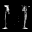
\includegraphics[scale=1]{tensors/sandc/valid/synth/Georgia-77} &
			
\includegraphics[scale=1]{tensors/sandc/valid/synth/Georgia-83} &
			
\includegraphics[scale=1]{tensors/sandc/valid/synth/VeraMoIt-86} &
			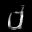
\includegraphics[scale=1]{tensors/sandc/valid/synth/VeraMoIt-100} &
			
\includegraphics[scale=1]{tensors/sandc/valid/synth/VeraMoIt-101} &
			
\includegraphics[scale=1]{tensors/sandc/valid/synth/VeraMono-66} &
			
\includegraphics[scale=1]{tensors/sandc/valid/synth/VeraMono-76} &
			
\includegraphics[scale=1]{tensors/sandc/valid/synth/VeraMono-89} 
		\end{tabu}
		\caption{Model output, having never seen these items during training.}
	\end{subfigure}
\caption[Style and Content generalisation]
{Example of images generated from unseen style and content pairs, three letters from
		 three different fonts.}
\label{fig:sandc-valid}
\end{figure}
\begin{figure}[hp]
	\begin{center}
	\begin{subfigure}[t]{0.45\textwidth}
		\centering
		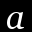
\includegraphics[scale=1]{tensors/sandc/valid/real/Georgiai-97}
		\caption{From the data}
	\end{subfigure}
	~
	\begin{subfigure}[t]{0.45\textwidth}
		\centering
		
\includegraphics[scale=1]{tensors/sandc/valid/synth/Georgiai-97}
		\caption{Generated}
	\end{subfigure}
	\end{center}
	\caption{A difficult example of style and content generalisation.}
	\label{fig:sandc-fail}
\end{figure}